\chapter{Synthesizing Data for the Detection of \ac{EWFO} on \acp{MAV}}


\section{Methodology}
\begin{figure}[htbp]
	\centering
	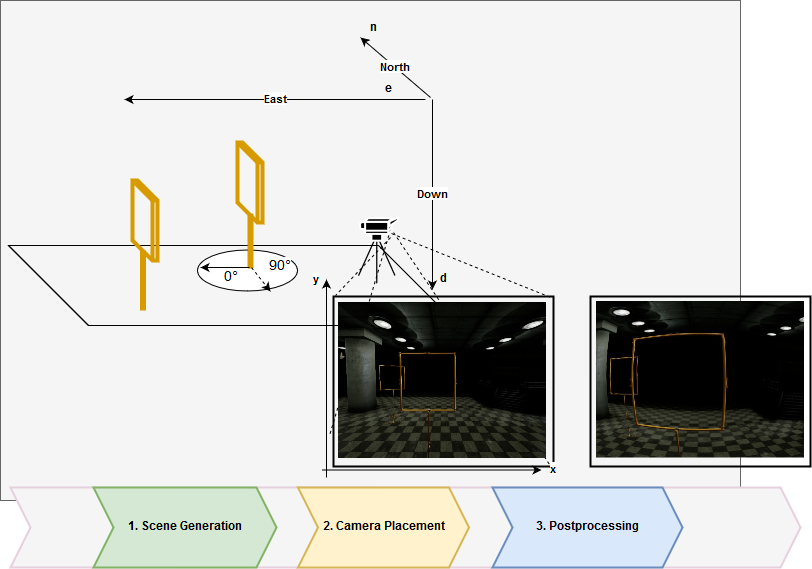
\includegraphics[width=0.9\textwidth]{fig/datagen_notation}
	\caption{Overview of the data generation process.}
	\label{fig:training:datagen_notation}
\end{figure}

In order to to investigate the research questions a data generation pipeline is implemented using OpenGL, UnrealEngine and AirSim. An overview can be seen in \Cref{fig:training:datagen_notation}. In the first step a scene is created in which the objects of interest as well as the camera are placed. In 3D space position and orientation (pose) of each object are determined by translation $\textbf{t}$ and rotation $\textbf{r}$. The coordinate system is \ac{NED}.

A view projection yields an image through the lens of the camera. The coordinates of each point in 3D space are projected on the 2D image plane. A final post processing step can simulate further effects like lens distortion and sensor noise. This step is implemented using OpenCV and Python.

All source code is made publicly available at \url{https://github.com/phildue/datagen.git}.

Within the pipeline environments for training and testing are created. A black environment serves as base to replace the background with existing images. Furthermore, three indoor base environments are created that fully simulate illumination and background. An overview can be seen in \Cref{fig:environments}. Within the environment light conditions, background textures, object locations can be changed manually. The environments are described in the following:

\begin{enumerate}
	\item \textit{Dark:} The environment is a room without windows, only containing artificial light sources. 
	\item \textit{Daylight:} The environment is a room with windows along all walls that allow daylight to illuminate the room. The windows can lead to strong variations in the contrast between different parts of the object.
	\item \textit{IROS:} The environment resembles the room of the \ac{IROS} Autonomous Drone Race 2018. The light sources stem from a window front at one side of the room, as well as artificial light sources at the ceiling. Depending on the view point, the object might appear against bright or dark background.
\end{enumerate}

\begin{figure}[hbtp]
	\centering
	\begin{minipage}{0.3\textwidth}
		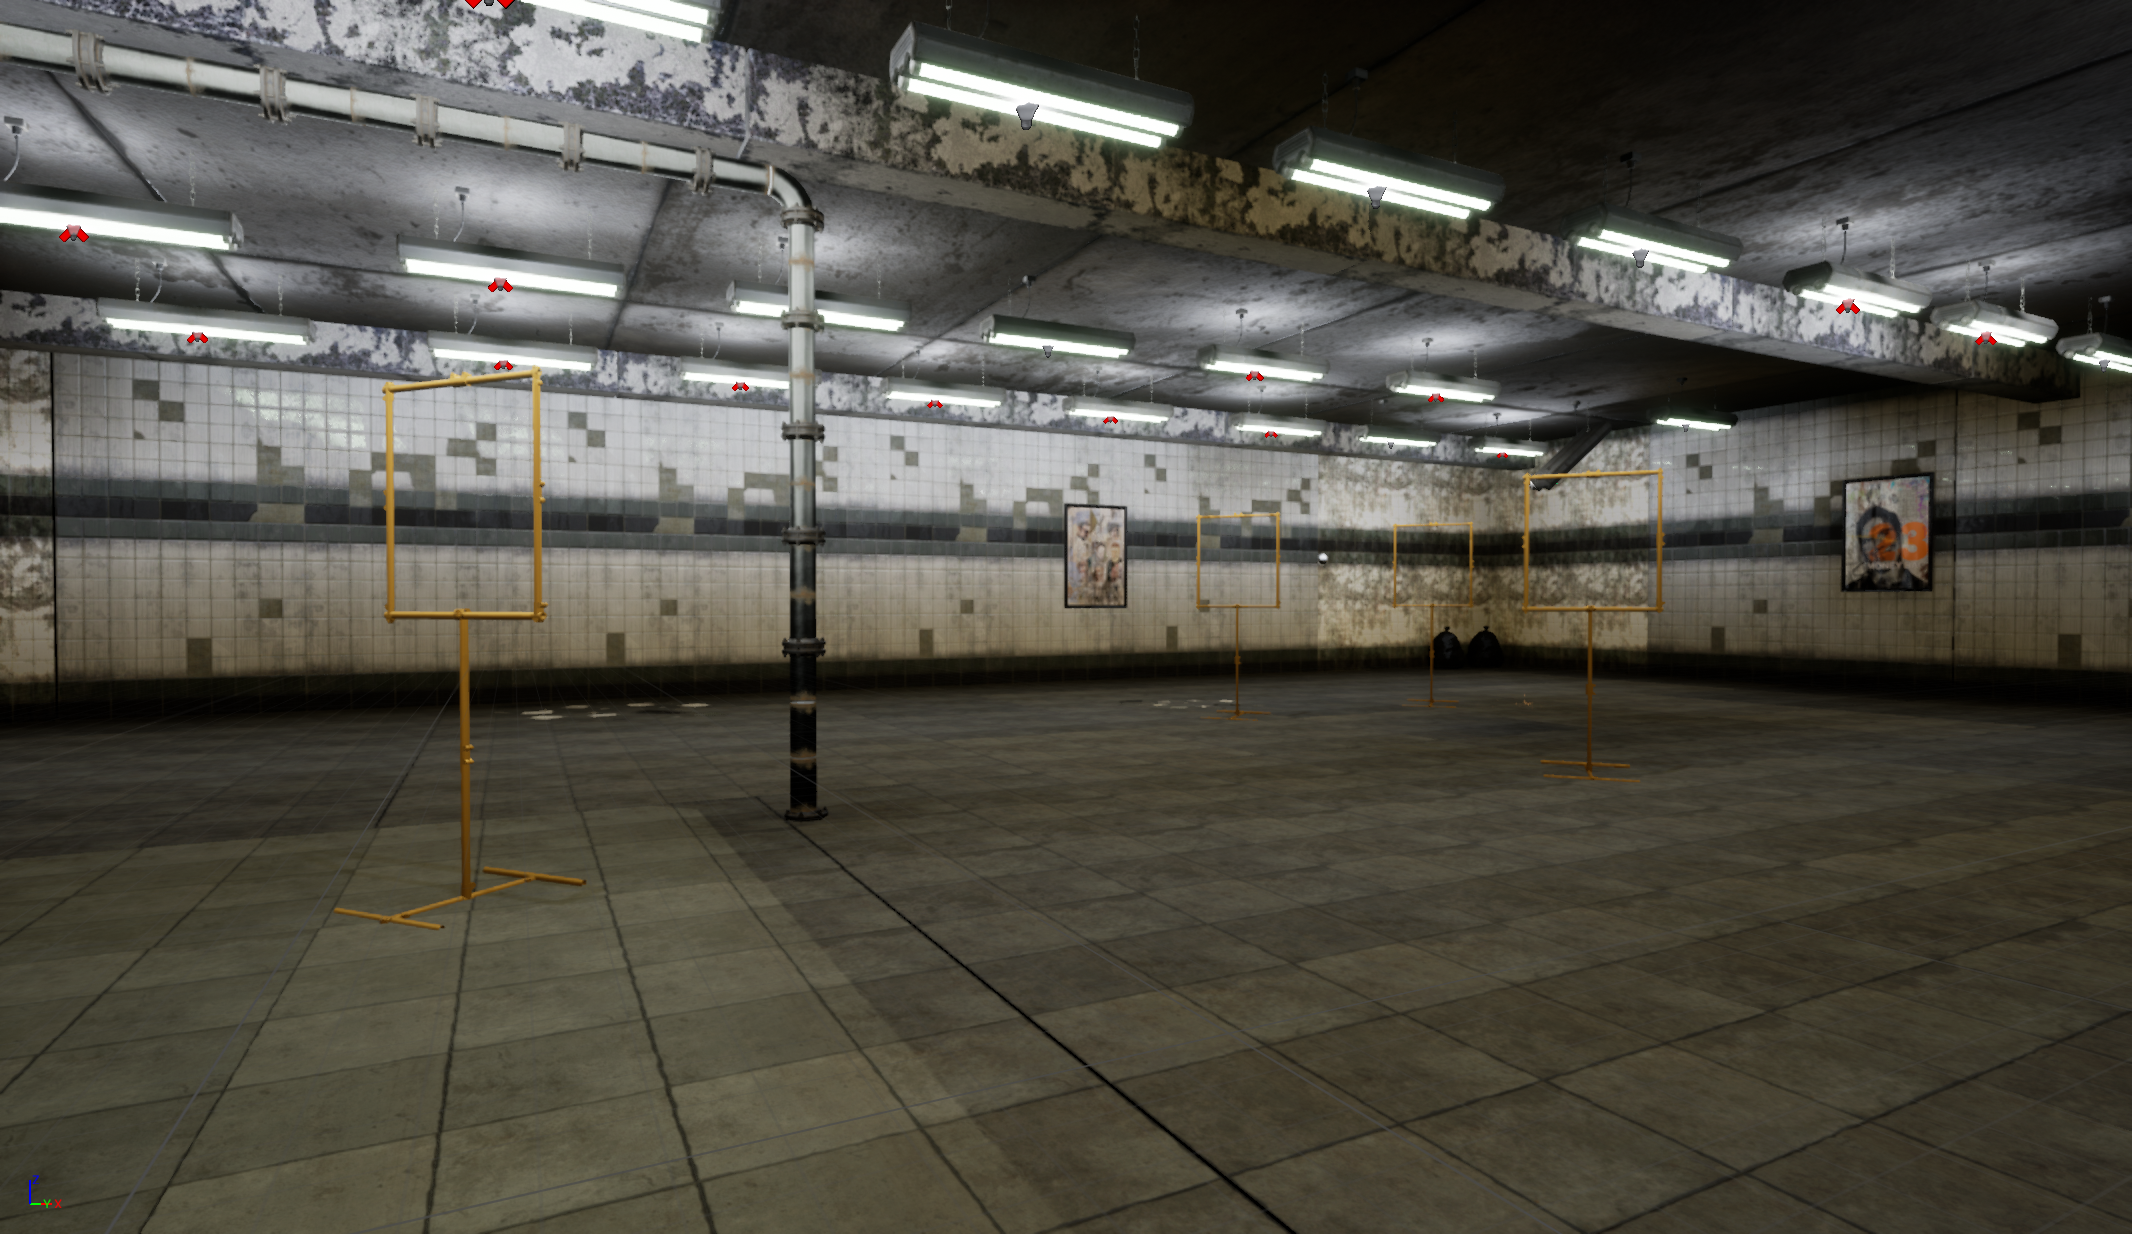
\includegraphics[width=\textwidth]{fig/basement_perspective}
	\end{minipage}
	\begin{minipage}{0.3\textwidth}
		\includegraphics[width=\textwidth]{fig/daylight_perspective}
	\end{minipage}
	\begin{minipage}{0.3\textwidth}
		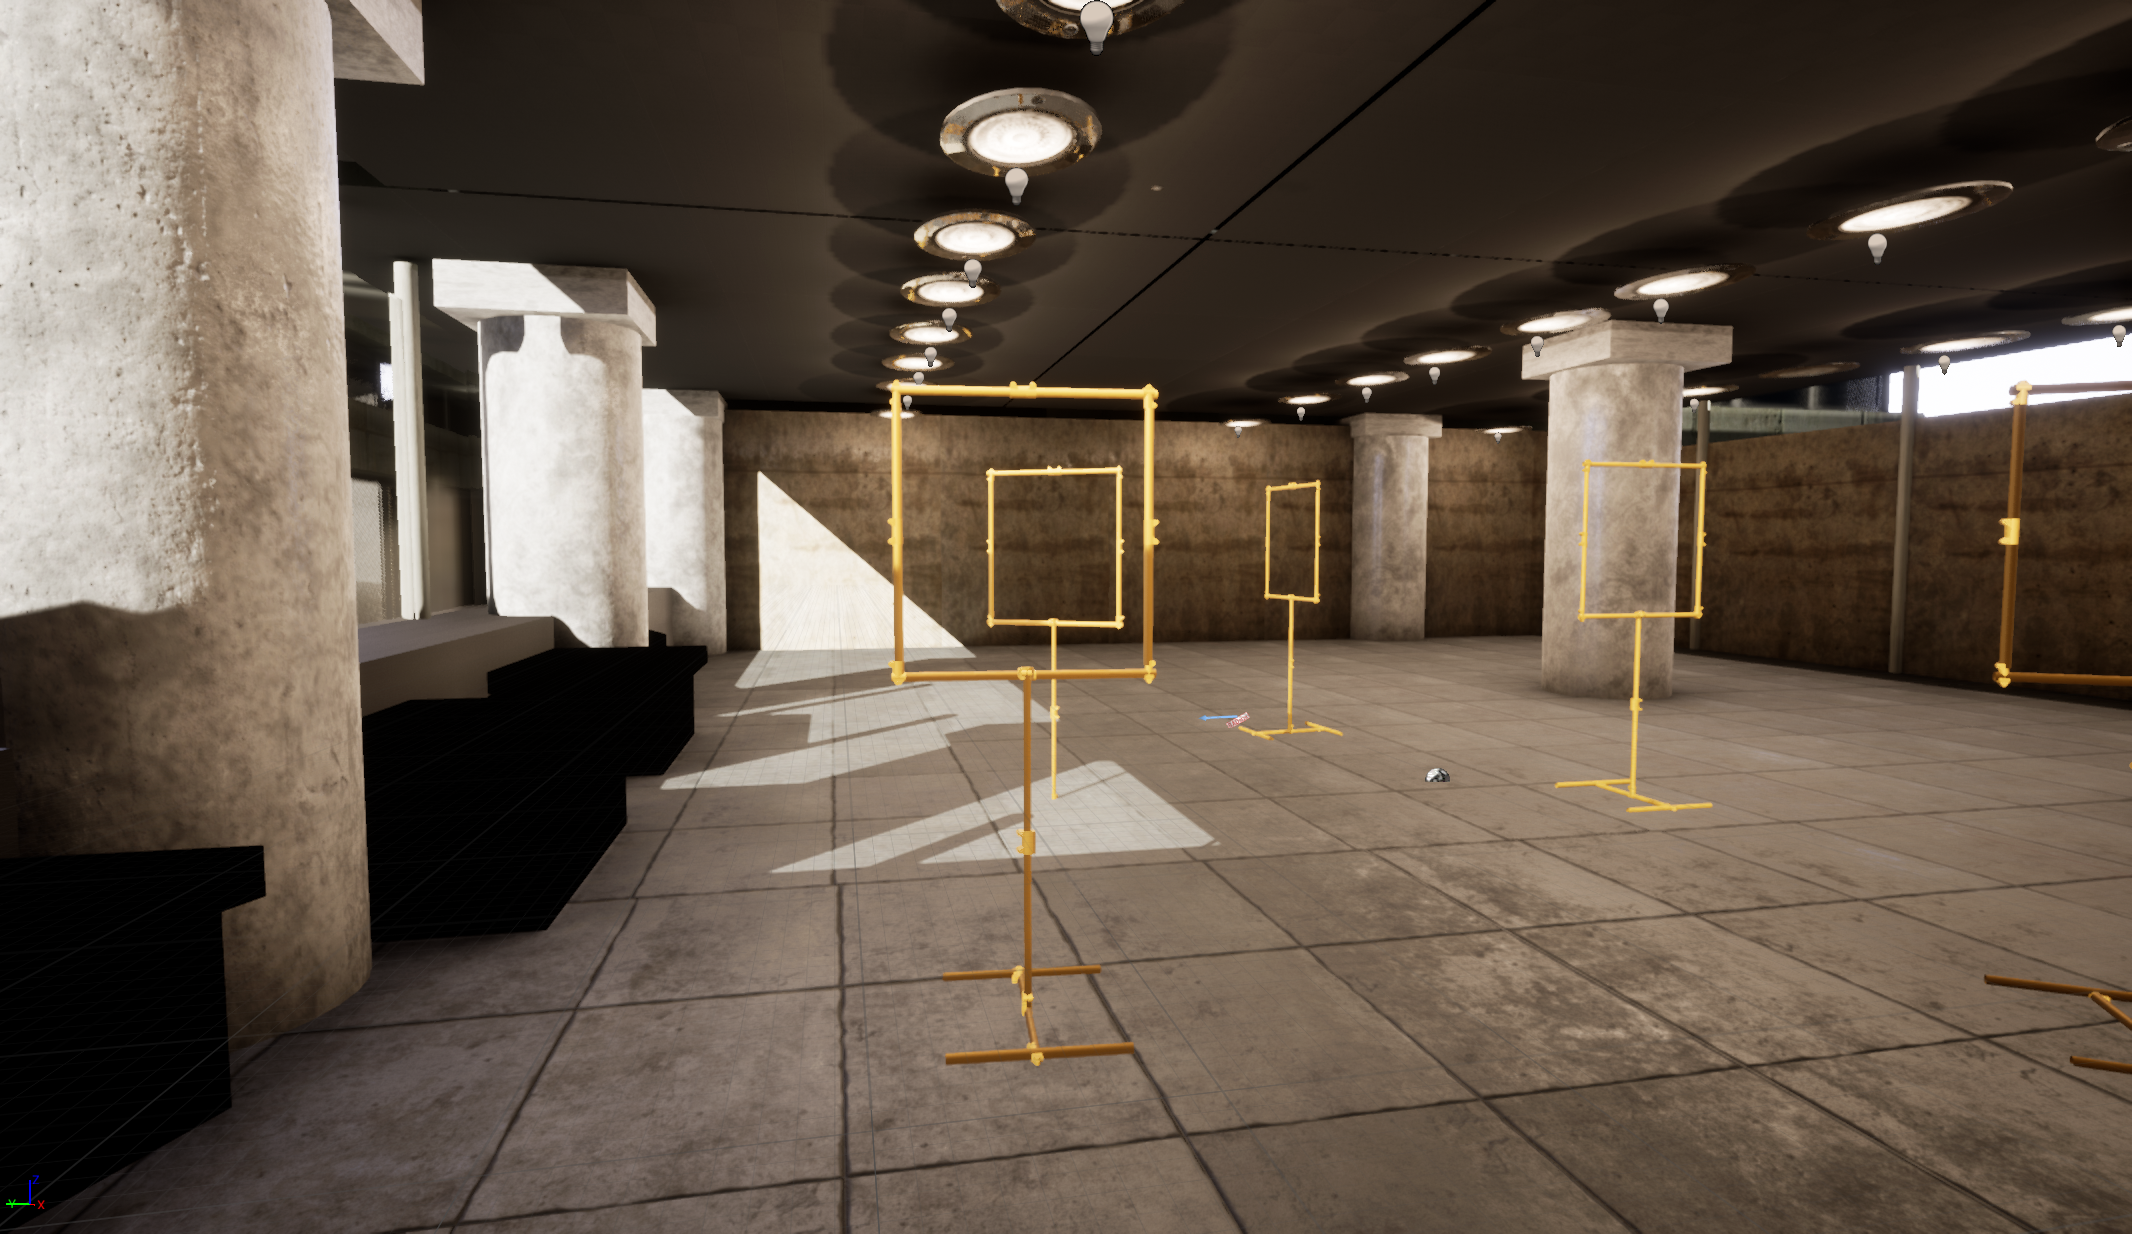
\includegraphics[width=\textwidth]{fig/iros_perspective}
	\end{minipage}
	\caption{\textit{IROS2018} Environment.}
	\label{fig:environments}
\end{figure}



It should be noted that when generating data with the described methods it is likely that samples appear in which only a corner of the object is visible or the view angle is in such a way that the object appears only as a thin line. In initial experiments these corner cases led to unstable training. Hence, some minimum requirements for the labels are set and samples are removed if these are not met. The criteria are:

\begin{itemize}
	\item Minimum Width/Height: 0.025 Image Width/Height
	\item Minimum Aspect Ratio: 0.3
	\item Maximum Aspect Ratio: 3.0
	\item Minimum Corners Visible: 3
\end{itemize}

\section{Context}

The context in which an object is placed consists of background as well as light conditions or other objects. It is determined in the first step of the data generation process. Theoretically \acp{CNN} can learn to exploit context for detection. Yet, the actual influence is not clear. For example the Object Detectors trained in \cite{Peng} do not seem to make use of this image cue. Nevertheless, we investigate the importance of context for the detection of \acp{EWFO}. We hypothesize that due to the sparsity of their features and their emptiness context and background plays a more important role than for solid objects.

For the investigation we compare three methods to generate data: The placement of \ac{CAD}-models on uniformly coloured backgrounds, on backgrounds taken from a dataset as well as from fully synthesized environments. In terms of geometric and physical properties the fully synthesized environments provide the most realism and hence should give the best results. However, as the graphical engine only contains a limited set of textures, the variance in background is way smaller than in the backgrounds taken from a dataset. Furthermore, the objects in the background are also rendered. Hence, when tested on real data this method could lead to better performance.

\subsection{Experiments}

Three datasets are generated with 20 000 samples each. Dataset I contains samples generated by placing \ac{CAD}-models on uniformly coloured backgrounds; Dataset II contains samples generated by placing \ac{CAD}-models on backgrounds taken from the Pascal VOC dataset, Dataset III contains samples generated by simulating a full environment.

Within the environment the camera is placed following these distributions:

\begin{equation}
x = \mathcal{U}(-30,30),\quad y = \mathcal{U}(-20,20),\quad z = \mathcal{N}(-4.5,0.5)),\quad
\phi = \mathcal{U}(0,0.1\pi),\quad \theta = \mathcal{U}(0,0.1\pi),\quad \psi = \mathcal{N}(-\pi,\pi)
\label{eq:distroexp}
\end{equation}

Where $ \mathcal{U}(a,b)$ is a uniform distribution between $a,b$ and $\mathcal{N}(\mu,\sigma^2)$ is a Gaussian distribution with mean $\mu$ and variance $\sigma^2$.


For each dataset the baseline TinyYoloV3-model is trained for 100 epochs using Adam optimizer and a learning rate of 0.001. 500 images are used as validation set and the training is stopped if the loss does not decrease for more than 5 epochs in a row. A fourth model is trained on a combination of Dataset II and III (equal proportion).

The models are tested on the real datasets as well as the simulated flight through the \textit{IROS} environment.


\subsection{Results}

\Cref{tab:context} and \Cref{fig:context} display the results. It can be seen how using uniformly coloured backgrounds achieve almost no performance. Only on the simulated data a few objects could be detected.

In contrast using fully synthesized data achieves the best performance on the simulated data for low and high quality detections. It can be seen that almost all detections have an \ac{IoU} of more than 60\% and are thus good quality. On the real data the performance in low quality detections is comparable to the performance on the simulated data. However, in hiqh quality detections the performance drops significantly to an equal level of using real backgrounds.

Using real backgrounds performs poorer than using a fully synthesized environment in almost every case. However, for higher quality detections the performance is competitive to using a fully synthesized environment.

Combining both methods does achieve at most the performance of using fully synthesized data. However, in most cases the performance is worse.   

\begin{table}[htbp]
	\caption{Results of different ways to generate context.}
\begin{tabular}{lrrrrrr}
	\hline
	Name &  Sim Data0.4 &  Sim Data0.6 &  Sim Data0.8 &  Real Data0.4 &  Real Data0.6 &  Real Data0.8 \\
	\hline
      Real Backgrounds &         0.26 &         0.15 &         0.02 &          0.14 &          0.09 &          0.01 \\
  Uniform Backgrounds &         0.04 &         0.02 &         0.00 &          0.00 &          0.00 &          0.00 \\
  Various Environments &         0.32 &         0.31 &         0.08 &          0.33 &          0.10 &          0.01 \\
        Real + Various &         0.32 &         0.18 &         0.04 &          0.12 &          0.10 &          0.01 \\
\hline
\end{tabular}
	\label{tab:context}
\end{table}

\begin{figure}[htbp]
	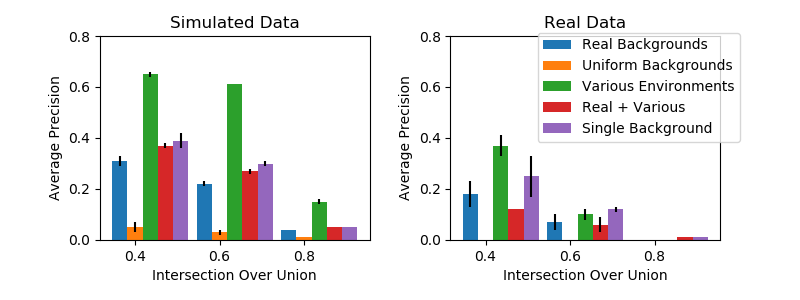
\includegraphics[width=\textwidth]{fig/context_bar}
	\caption{Results of different ways to generate context. Synthesizing more parts of the environment improves performance on both test sets. However, this only holds for weakly localized predictions.}
	\label{fig:context}
\end{figure}

\subsection{Discussion}

The results meet our hypothesis that using only uniformly coloured backgrounds is not enough to train an Object Detector for \ac{EWFO}. Providing more variance in the background is crucial to improve performance.

Despite having not seen a single real background, the model trained on fully synthesized data achieves the best performance on the real data. Hence, it seems that synthesizing correct geometric/physical properties is more important than providing a large variance in background.

However, the margin gets small for higher quality detections. Thus, the simulation of geometric/physical properties does not help for good localization.

\subsection{Conclusion}

We can conclude that providing a realistic environment benefits the detection.

\section{View}

Another important property that influences the generated sample is the camera pose. It determines the view on the scene and therefore at which distance, angle and location the objects appear on the image.

A straightforward way is placing the camera randomly (within some margin) in order to cover a large variation of views on the object. That way the network can learn a general object representation and hopefully detect unseen objects from different view points. However, random a placement might not resemble the real world sufficiently. An \ac{MAV} does not appear at random places within a scene, especially not when it follows a racing track. We examine this by simulating a flight through a race court using AirSim's \ac{MAV} model and analyzing the relative object poses. We compare these to the relative poses obtained when placing the camera randomly using the distributions from \Cref{eq:distroexp}.

\begin{figure}
	\begin{minipage}{\textwidth}
		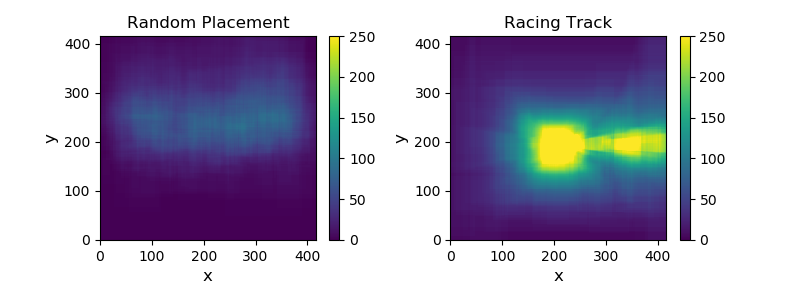
\includegraphics[width=\textwidth]{fig/heatmap_camplace}
		\caption{Object appearances when generating samples with random poses (left) and during a \ac{MAV} flight. During the flight the object appears mostly centered on the horizontal line.}
		\label{fig:heatmap_camplace}
	\end{minipage}
	\begin{minipage}{\textwidth}
		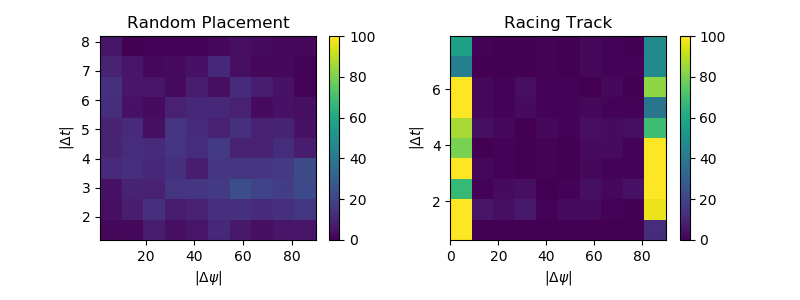
\includegraphics[width=\textwidth]{fig/hist2d_camplace}
		\caption{Histogram of object occurrences in yaw angle and distance relative to the camera. The random placement does rarely cover facing the object closely and frontally. }
		\label{fig:hist2d_camplace}
	\end{minipage}
\end{figure}

\Cref{fig:heatmap_camplace} shows the distribution of bounding boxes when created with random camera placement and when following a racing track. It can be seen how, when following the race track most of the objects are centered and distributed across the horizon, as camera focuses the next object frontally most of the time. In contrast, random placement leads to more evenly distributed object locations. This can also be seen in \Cref{fig:hist2d_camplace} where a 2D histogram of the yaw angle and distance with respect to the camera is displayed. Thereby 0 corresponds to facing the object frontally, 180 degrees facing the object from the back. It is apparent how the random placement covers a much larger range of relative angles, while in the racing track certain angles do not appear at all. Even more importantly the largest bins of the racing track is an angle of 0 and a distance between 0m and 4m. These bins are almost not present when placing the camera randomly. This is because close to the camera the field of view is small, while the area of the object faced frontally is big. Hence, the probability of an object ending up at this specific location is relatively low. Furthermore, when placing the camera randomly there are no samples further away than 8m. This is because in the race track the camera traverses the room from one end - where it can see almost all gates - to another. The probability that the randomly placed camera ends up in a similar position is relatively low.

The filters of \acp{CNN} are translation invariant by design but cannot inherently handle variation in rotation and scale. We hypothesize that the generation of samples with only one of the two methods can miss important object appearances. Random placement does not cover appearances that are typical for a autonomous drone race. On the other hand, only training on racing tracks might lead to a bias towards the created courses.

\subsection{Experiments}

In order to to evaluate this hypothesis three models are trained on 20 000 samples each. Model I is trained when placing the camera randomly, following the distribution in \Cref{eq:distroexp}. Model II is trained on varying racing courts. Model III is trained on a combination of both datasets (equal proportion).

The models are tested on the real datasets as well as the simulated flight through the \textit{IROS} environment.

\subsection{Results}

\begin{figure}[htbp]
	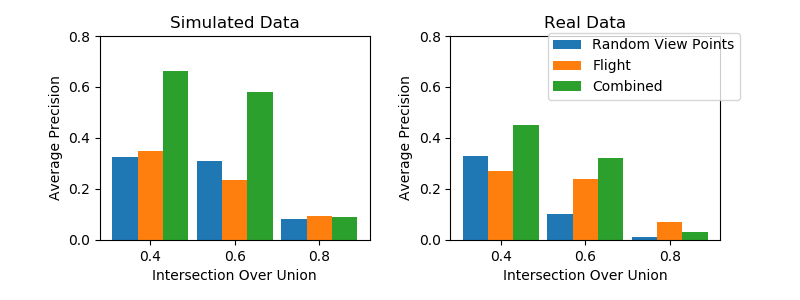
\includegraphics[width=\textwidth]{fig/view_bar}
	\caption{Performance across clusters.}
	\label{fig:view_bar}
\end{figure}

\Cref{fig:view_bar} shows the average precision of the different models. It should be noted that \textit{Random View Points} is the same model as \textit{Various Environments} of \Cref{fig:context}. It can be seen how Model I and Model II perform comparable on the simulated dataset. In contrast on the real dataset the performance in high quality detections is significantly better when training the network on flight images.

Combining both datasets improves the performance mainly on lower quality detections. This holds particularly for low detections with lower bounding box accuracy.

\todo{combined}

\begin{figure}[htbp]
	\centering
	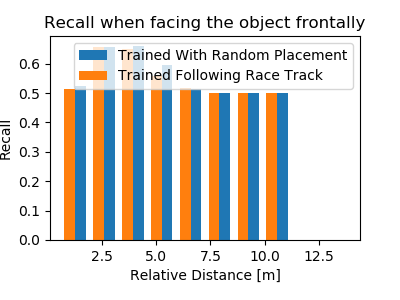
\includegraphics[width=\textwidth]{fig/recall_front}
	\caption{Performance when facing the object frontally.}
	\label{fig:recall_front}
\end{figure}

\begin{figure}[htbp]
	\centering
	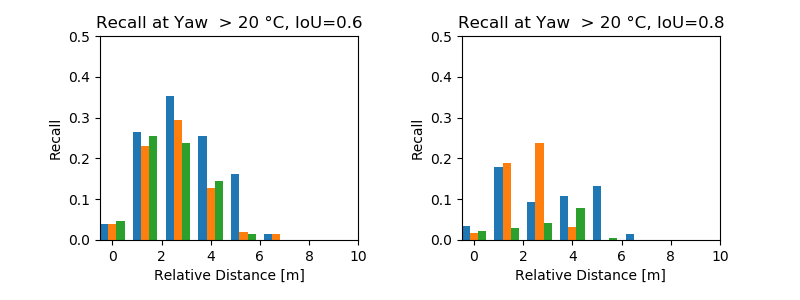
\includegraphics[width=\textwidth]{fig/recall_angle}
	\caption{Performance when facing the object frontally.}
	\label{fig:recall_angle}
\end{figure}

\Cref{fig:recall_front} and \Cref{fig:recall_angle} show the performance of different models in terms of recall. It can be seen how for a lower quality detections the performance of the model trained on random view points is slightly better than when training the network on simulated flight images. However, for high quality detections the model trained on flight images achieves a higher recall for objects that are close to the camera. This holds even for objects that are not faced frontally. Yet for higher distances the model trained on random view points achieves a higher recall. Generally, it can be seen that the recall first increases when moving the object away from the camera before it decreases again.

\begin{figure}[htbp]
	\centering
	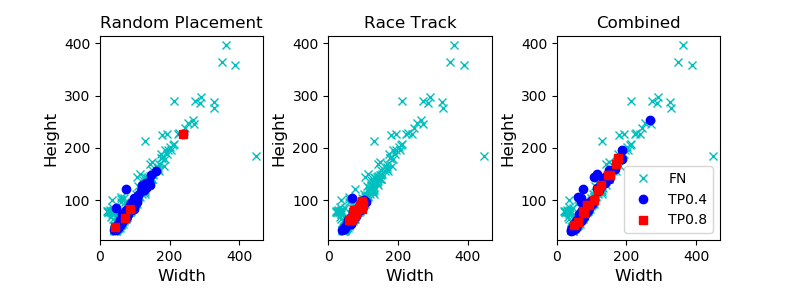
\includegraphics[width=\textwidth]{fig/view_scatter}
	\caption{Performance when facing the object frontally.}
	\label{fig:view_scatter}
\end{figure}

\subsection{Discussion}

Even though one model is trained on various race courts it cannot be said it also performs better when applied on a race court. It looks like the recall for high quality predictions increases for the view points that are more present in the training domain. However, an significant difference in the overall performance cannot be identified. The reason could be the model trained on racing tracks is biased towards the respective view points. Hence, it performs very well when objects appear at the same location. Yet this performance comes at cost of generalization, the recall for other objects decreases. The models trained on random view points or a combined dataset have to cover a large variance in object appearance. While this leads to more detections, the bounding boxes for these detections are less accurate. 

It can also be observed that the performance for objects that are close to the camera are quite poor. This is potentially explained by the fact that less object context is available. For example the pole for closer objects is less visible. Also, the probability of having a part of the object out of view increases as the camera comes closer. Another issue could be the limited receptive field of the detection model. YoloV3 assigns the responsibility of an output node based on the \ac{IoU} with the ground truth. However, when \ac{EWFO} are empty and spread over a large area, thus it is possible that the responsible node does not see a feature of the object it is assigned to detect.

For larger distances the performance decreases again. This is explained by the fact that less details of the objects are visible as the camera moves further away.

\todo{more context when farer away}

\subsection{Conclusion}


\section{Post-processing}

After having created a set of 2D images, the final step applies low-level image transformations. It allows to further simulate sensor effects and increase the variance in the generated data.

In literature \cite{Krizhevsky2012a,Howard2013,Redmon,Liu} the application of image augmentation is a common tool to improve the detection performance. The experiments in \cite{Carlson2018} show how the incorporation of sensor effects particularly improves the performance of models learned on fully synthesized data. In the \ac{MAV} domain sensor and lens effects have a significant influence on the obtained sample. Hence, we hypothesize that the incorporation of these effects is particularly useful for the \ac{MAV} domain.

\paragraph{Lens Distortion}

Lens distortion is a form of optical aberration which causes light to not fall in a single point but a region of space. For \acp{MAV} commonly used wide-angle lenses, this leads to barrel distortion and thus to straight lines appearing as curves in the image.

The effect is applied using the model for wide-angle lenses from \cite{Vass}. It models the removal of lens distortion as combination of radial and non-radial part, that is approximated with a second order Taylor expansion:
\todo{double check formula is (y in first line?)}
\begin{equation}
f(x,y) =
\begin{pmatrix}
x (1 + \kappa_1 x^2 + \kappa_1 (1 + \lambda_x) y^2 + \kappa_2(x^2 + y^2)^2) \\
y (1 + \kappa_1 x^2 + \kappa_1 (1 + \lambda_y) y^2 + \kappa_2(x^2 + y^2)^2)
\end{pmatrix} 
\label{eq:distortion}
\end{equation}
Where:
\begin{itemize}
	\item f yields the undistorted coordinates.
	\item $\kappa_1$ $\kappa_2$ control the radial distortion 
	\item $\lambda_x$ and $\lambda_y$ control the tangential distortion
\end{itemize}

Applying the lens distortion to an image is done using the inverse of \Cref{eq:distortion}. However, as there is no closed form solution, so the Newton-approximation.

An example with $\kappa_1 = 0.5, \kappa_2 = 0.5$ is displayed in \Cref{fig:distortion}. It can be seen how the previously straight lines appear as circular shape.

\paragraph{Chromatic Aberration.}

Chromatic Aberration is caused when different wavelengths of light do not end up in the same locations of the visual sensor. This leads to a shift in the colour channels of the image.

Similarly to \cite{Carlson2018}, chromatic aberration is applied by scaling the locations of the green channel, as well as applying translations on all channels. The model can be implemented as affine transformation of the pixel locations for each channel:

\begin{equation}
f(x_C,y_C) = \begin{pmatrix}
S & 0 & t_x \\
0 & S & t_y \\
0 & 0 & 1
\end{pmatrix} \begin{pmatrix}
x_C \\
y_C \\
1
\end{pmatrix}
\end{equation}

Where $C$ is one colour channel of the image.

An example is displayed in \Cref{fig:chromatic}. It can be seen how the red and green channel are shifted relative to each other. Thus two bars appear in the image.

\paragraph{Blur}

Motion noise is caused when light falls in different locations of the images sensor due to a fast movement of the camera. It leads to blurry images based on the sensor motion.

The phenomenon depends on camera properties as well as the motion of camera and objects. Although a full modelling of this process might benefit the learning process, it requires a complex pipeline and is computationally expensive. Therefore a strong simplification is used, namely a one-dimensional Gaussian filter:

An example for vertical blur is displayed in \Cref{fig:motionblur}. It can be seen how particularly horizontal lines appear softer.

Next to motion, sensor noise can lead to blurry images. For the blur operation a 2D Gaussian kernel is applied on the input image with:

\begin{equation}
k = \frac{1}{2\sigma_x\sigma_y\pi}e^{-\sqrt{\frac{x^2 + y^2}{2\sigma_x\sigma_y}}} 
\end{equation}
\todo{double check notation}
\paragraph{Exposure.}

Exposure is the time the sensor records light in order to create an image. Over- and Underexposure are caused when this time is too short or too long, leading to too dark or too bright images.

Following the model from \cite{Carlson2018}:

\begin{equation}
f(S) = \frac{255}{1 + e^{-A S}}
\end{equation}
where $A$ is a constant term for contrast and $S$ the exposure.
\todo{whats a}
The image can be re-exposed with:

\begin{equation}
I' = f(S+\Delta S)
\end{equation}

where $S$ is obtained from :
\begin{equation}
S = f^{-1}(I)
\end{equation}

An example for overexposure is displayed in \Cref{fig:exposure}. It can be seen how lighter areas appear particularly light, while dark areas remain dark.

\paragraph{Color Variations}

\todo{describe hsv scaling}


\begin{figure}[htbp]
	\centering
	\begin{minipage}{0.33\textwidth}
		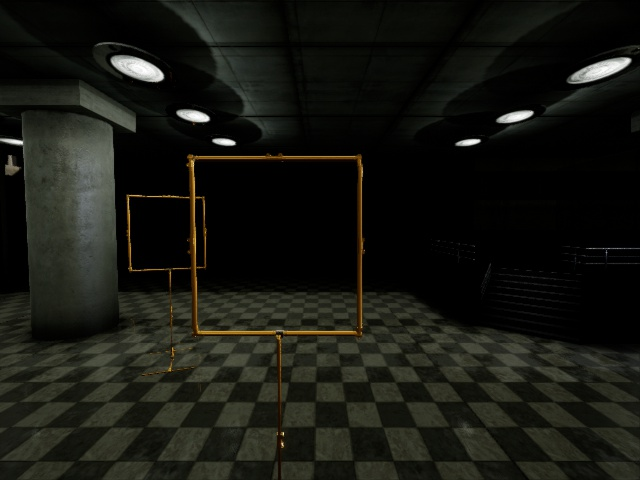
\includegraphics[width=\textwidth]{fig/gate_example}
		\caption{Original Image.}
		\label{fig:orig}
	\end{minipage}
	\begin{minipage}{0.33\textwidth}
		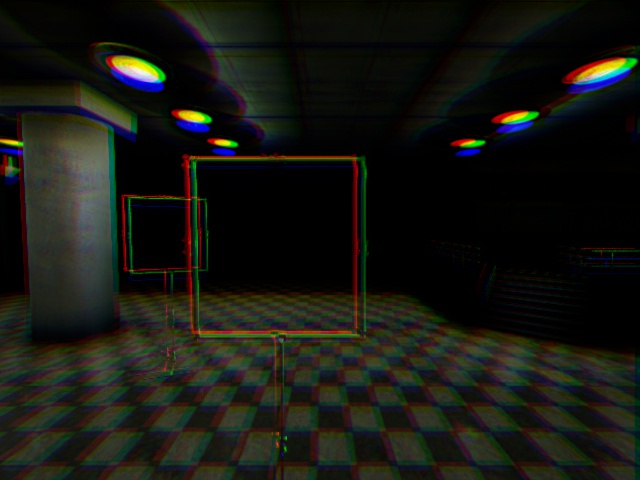
\includegraphics[width=\textwidth]{fig/gate_example_chromatic}
		\caption{Chromatic Aberration.} 		
		\label{fig:chromatic}
	\end{minipage}
	\begin{minipage}{0.33\textwidth}
		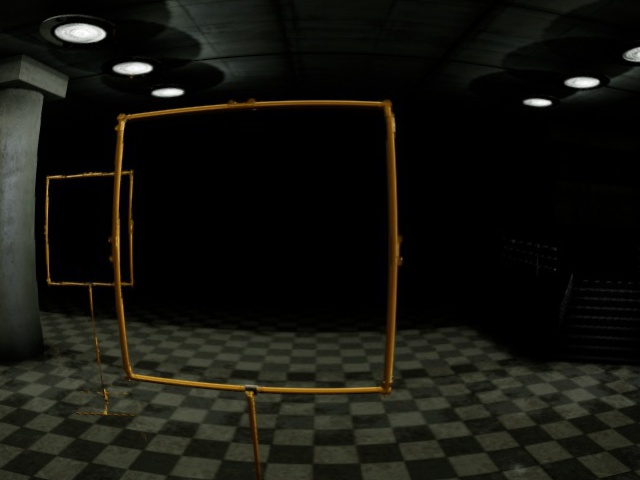
\includegraphics[width=\textwidth]{fig/gate_example_distorted}
		\caption{Lens Distortion. }		
		\label{fig:distortion}
	\end{minipage}
	
	\begin{minipage}{0.33\textwidth}
		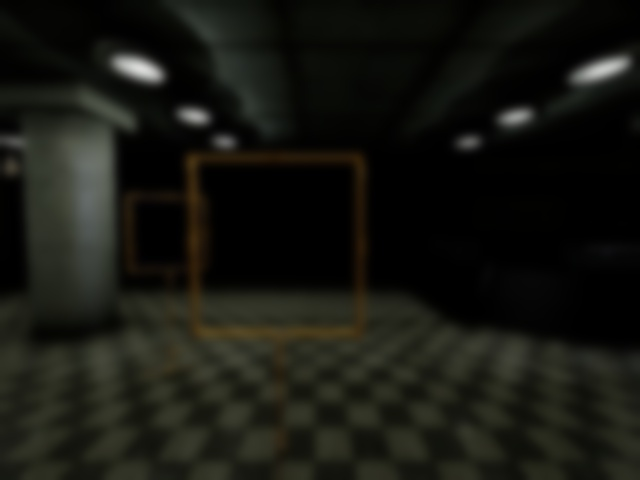
\includegraphics[width=\textwidth]{fig/gate_example_focusblur}
		\caption{Out-of-Focus blur.}
		\label{fig:focusblur}
	\end{minipage}
	\begin{minipage}{0.33\textwidth}
		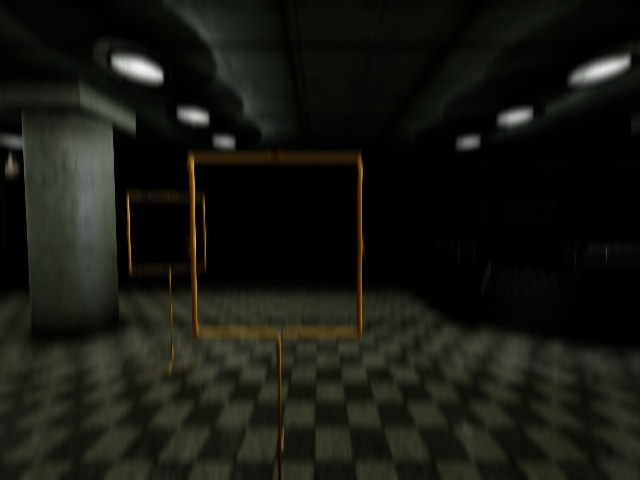
\includegraphics[width=\textwidth]{fig/gate_example_motionblur_v}
		\caption{Vertical Motion Blur.}
		\label{fig:motionblur}
	\end{minipage}
	\begin{minipage}{0.33\textwidth}
		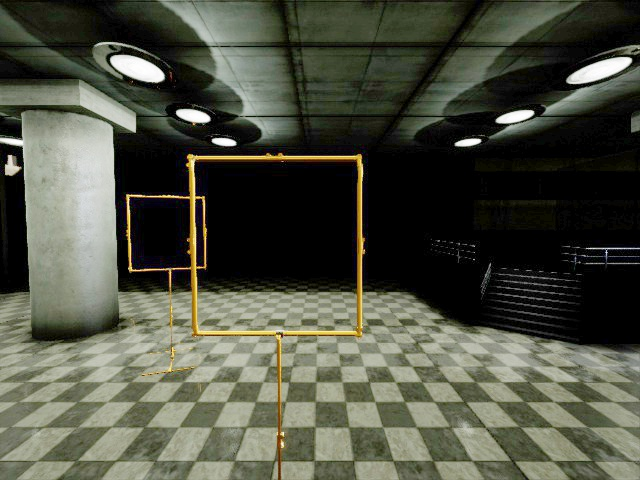
\includegraphics[width=\textwidth]{fig/gate_example_exposure}
		\caption{Exposure.}
		\label{fig:exposure}
	\end{minipage}
\end{figure}



\subsection{Experiments}

\subsubsection{Background}

The empty space of an \ac{EWFO} is augmented with a detailed texture. An example can be seen in \Cref{fig:cats}.
\begin{figure}
	\centering
	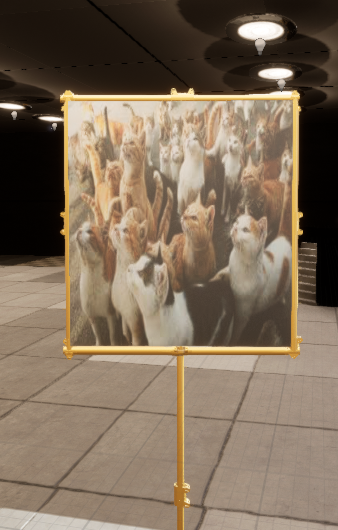
\includegraphics[height=5cm]{fig/cat}
	\caption{The \ac{EWFO} is augmented with a detailed texture.}
	\label{fig:cats}
\end{figure}

The object is placed in a scene with uniformly coloured backgrounds and a training set of 20 000 samples is created. In similar fashion a training set is created without the texture rich augmentation. The test set contains 1000 samples created in the \textit{IROS} environment by randomly placing the camera following \Cref{eq:distroexp}.


\subsubsection{Context}

Several models are trained on 20 000 samples each.
\begin{itemize}
	\item[ModelU] Uniform
	\item[ModelSVE] Single Virtual Environment
	\item[ModelRB] Real Backgrounds
	\item[ModelVVE] Various Virtual Environments
	\item[ModelRBVVE] Real Backgrounds + Various Virtual Environments
\end{itemize}


\begin{table}[htbp]
	\caption{}
	\begin{tabular}{|l|l|l|l|r|r|r|l|l|l|}
		\hline
		& Validation Set &  &  & \multicolumn{1}{l|}{IROS2018} & \multicolumn{1}{l|}{} & \multicolumn{1}{l|}{} & Real Data &  &  \\ \hline
		& AP40 & AP60 & AP80 & \multicolumn{1}{l|}{AP40} & \multicolumn{1}{l|}{AP60} & \multicolumn{1}{l|}{AP80} & AP40 & AP60 & AP80 \\ \hline
		U &  &  &  & 0.05 & 0.01 & 0 &  &  &  \\ \hline
		SVE &  &  &  & 0.29 & 0.17 & 0.02 &  &  &  \\ \hline
		VVE &  &  &  & 0.61 & 0.49 & 0.17 &  &  &  \\ \hline
		RB &  &  &  & 0.42 & 0.28 & 0.04 &  &  &  \\ \hline
	\end{tabular}
	\label{tab:env}
\end{table}


\subsubsection{View}


\subsubsection{Discussion}

\subsubsection{Conclusion}


\subsection{Hypothesis}
\label{sec:training:hypothesis}

This chapter summarizes the hypotheses formulated in the previous chapters:

\begin{enumerate}
	\item[$\mathcal{H}_1$] An object that is not empty and provides a more distinctive structure is less background dependent than an \ac{EWFO}.
	
	\item[$\mathcal{H}_2$] The incorporation of correct placement/light conditions improves the performance of a model trained to detect \acp{EWFO}.
	
	\item[$\mathcal{H}_3$] The incorporation of a camera motion model resembling the target domain improves the performance of a model trained to detect \acp{EWFO}. 
	
	\item[$\mathcal{H}_3$] Including sensor effects present in the target domain, improves the performance of a model trained to detect \acp{EWFO}. 
	
\end{enumerate}



\section{Experiments}
\label{sec:training:experiments}
In order to evaluate the formulated hypotheses several experiments are conducted. The model used is the TinyYoloV3-Architecture, further described in \Cref{sec:object_detection}. The reported metrics are described in \Cref{sec:metrics}. For all experiments mean and standard deviation of 5 runs are reported.

For the random view point generation the following parameters are used:


Where $ \mathcal{U}(a,b)$ is a uniform distribution between $a,b$ and $\mathcal{N}(\mu,\sigma^2)$ is a Gaussian distribution with mean $\mu$ and variance $\sigma^2$.

The parameters are chosen experimentally aiming to resemble common view points of a person standing in the room.

\subsubsection{Experiment I}


\subsubsection{Experiment II}



\subsubsection{Experiment III}

Three models are trained: Model I using random placement, Model II using the drone motion model, Model III using a combination of both methods. In both experiments environment and light conditions as well as object locations are the same. The models are tested on two test sets: Set I created by randomly placing the camera. Set II by using the drone motion model, where a circuit is used that has not been part in the generation of the training data.


\subsubsection{Experiment IV}

In order to evaluate $\mathcal{H}_4$ the individual domain properties are measured on the target domain and incorporated in the training set.


\section{Results}
\label{sec:training:results}

\section{Discussion}
\label{sec:training:discussion}

\section{Conclusion}
\label{sec:training:conclusion}
